\chapter{Experimental Setting}

The current chapter is divided into two sections. In the first one we will describe the benchmark of the experiment regarding the creation of the RL agent and its results. In the second one we will describe the same experiment applied to humans and its results.

\section{Benchmark}

\paragraph{Test Functions}

As already explained, the experiment described in this work is about maximization a black-box function adopting an RL based approach. The first important choice is about selecting suitable \textit{test functions}. In applied mathematics, test functions, known as \textit{artificial landscapes}, are useful to evaluate characteristics of optimization algorithms. In this thesis we have chosen four test functions:

\begin{itemize}
	\item Himmelblau' s Function;
	\item Parabolic Function;
	\item Beale Function;
	\item Styblinski Function.	
\end{itemize}

\subparagraph{Parabolic Function} In mathematical optimization, Himmelblau' s function is a multi-modal function introduced by David Mautner Himmelblau (1924–2011). The function is defined by: 

\begin{equation}
	f(x, y) = (x^2 + y -11)^2 + (x + y^2 - 7)^2
\end{equation}

It has a local maximum at $x = -0.270845$ and $y = -0.923039$ where $f(x, y) = 181.617$, and four local minima :

\begin{itemize}
	\item $f(3.0, 2.0) = 0.0$;
	\item $f(-2.805118, 3.131312) = 0.0$;
	\item $f(-3.779310, -3.283186) = 0.0$;
	\item $f(3.584428, -1848126) = 0.0$.
\end{itemize}
	
It's domain is $x = (-5, 5)$ and $y = (-5, 5)$.

\begin{figure}[h!]
	\centering
	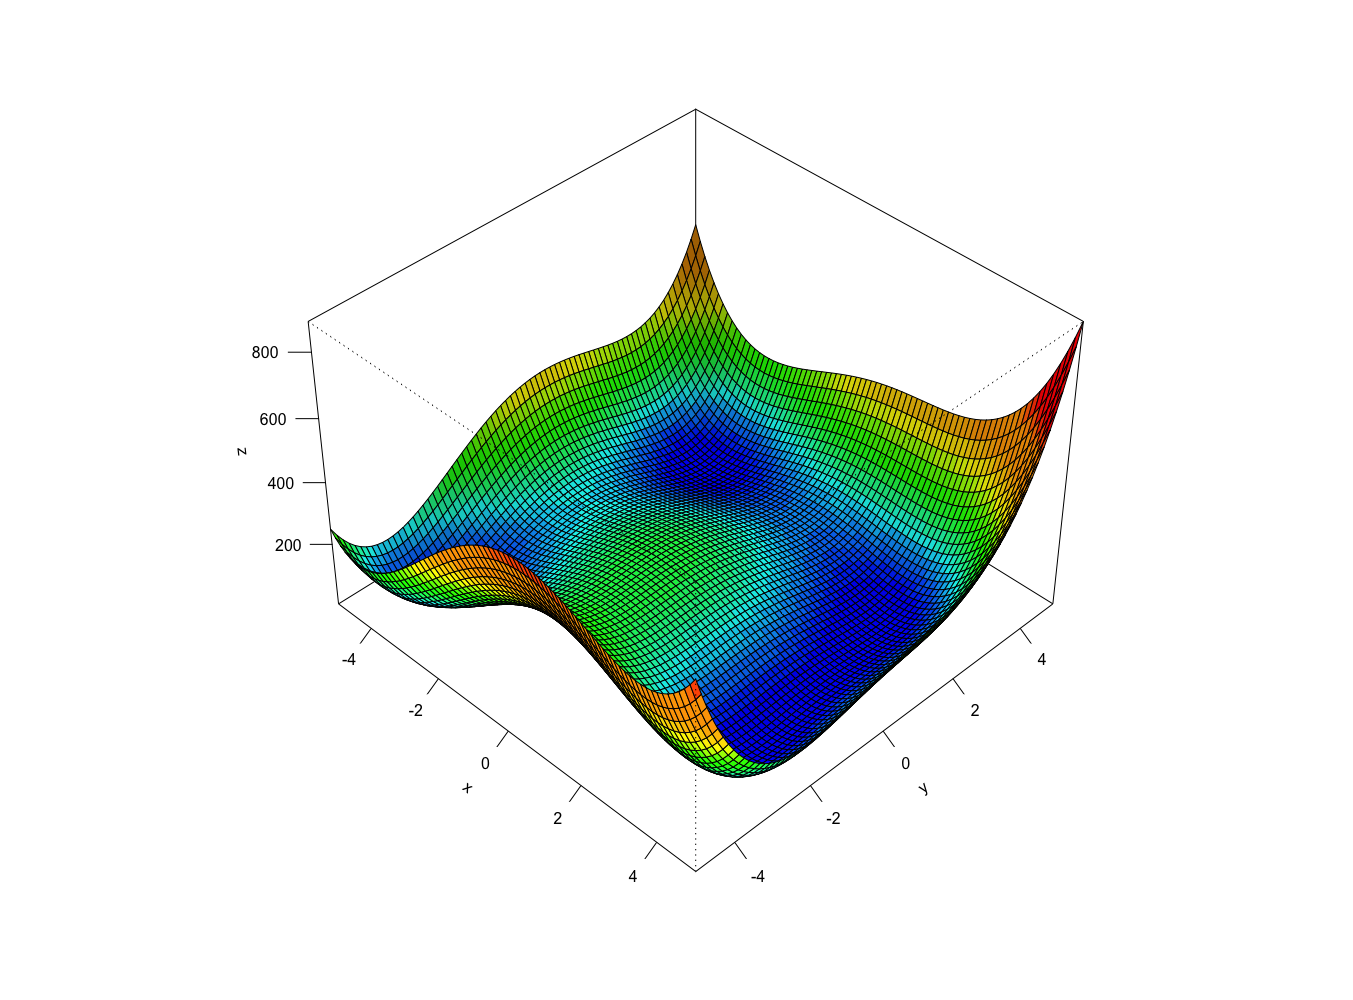
\includegraphics[width= 14cm, height = 12cm]{originalHimmelblau.png}
	\caption{Original Himmelblau Function.}
	\label{fig:OriginalHimmelblauFunction}
\end{figure}

In this thesis our aim is to maximize. In order to do this we have inverted the function as follow :

\begin{equation}
f(x, y) = -(x^2 + y -11)^2 + (x + y^2 - 7)^2
\end{equation}

and we have picked it up of $2500$ units in order to have as less as possible negative values. So the final adopted function is :
 
\begin{equation}
f(x, y) = -(x^2 + y -11)^2 + (x + y^2 - 7)^2 + 2500
\end{equation}

\begin{figure}[h!]
	\centering
	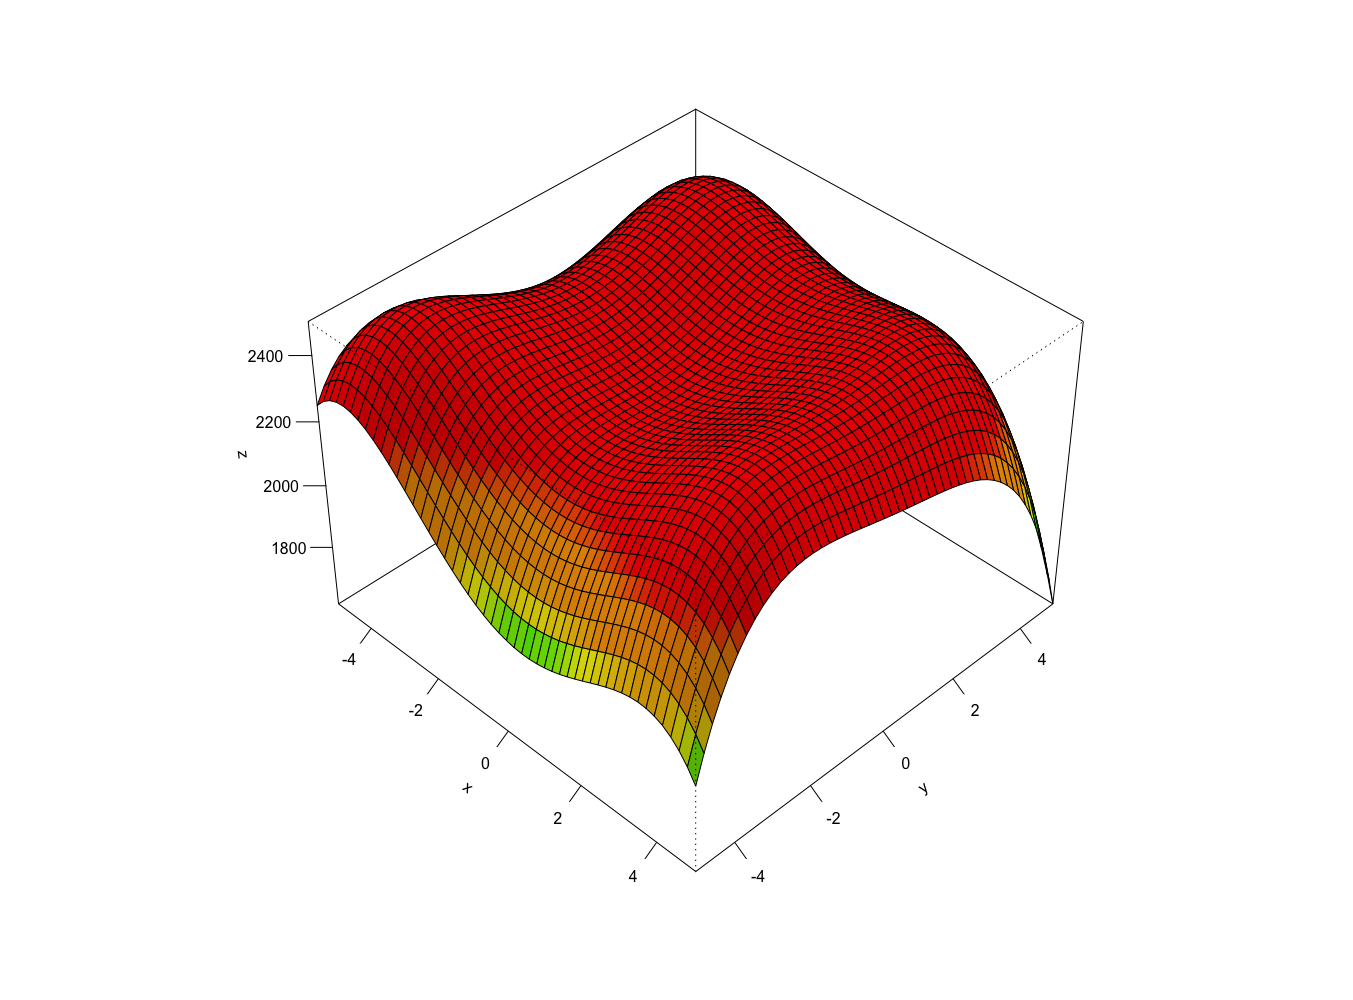
\includegraphics[width= 14cm, height = 12cm]{modifiedHimmelblau.png}
	\caption{Customized Himmelblau Function.}
	\label{fig:CustomizedHimmelblauFunction}
\end{figure}

In order to represent this function using {\tt JPanel} we mapped it in a space of $600 \times 600$ pixels and we properly rotated it. The resulting contour plot is the one represented in figure ~\ref{fig:ContourPlotCustomizedHimmelblauFunction} 

\begin{figure}[h!]
	\centering
	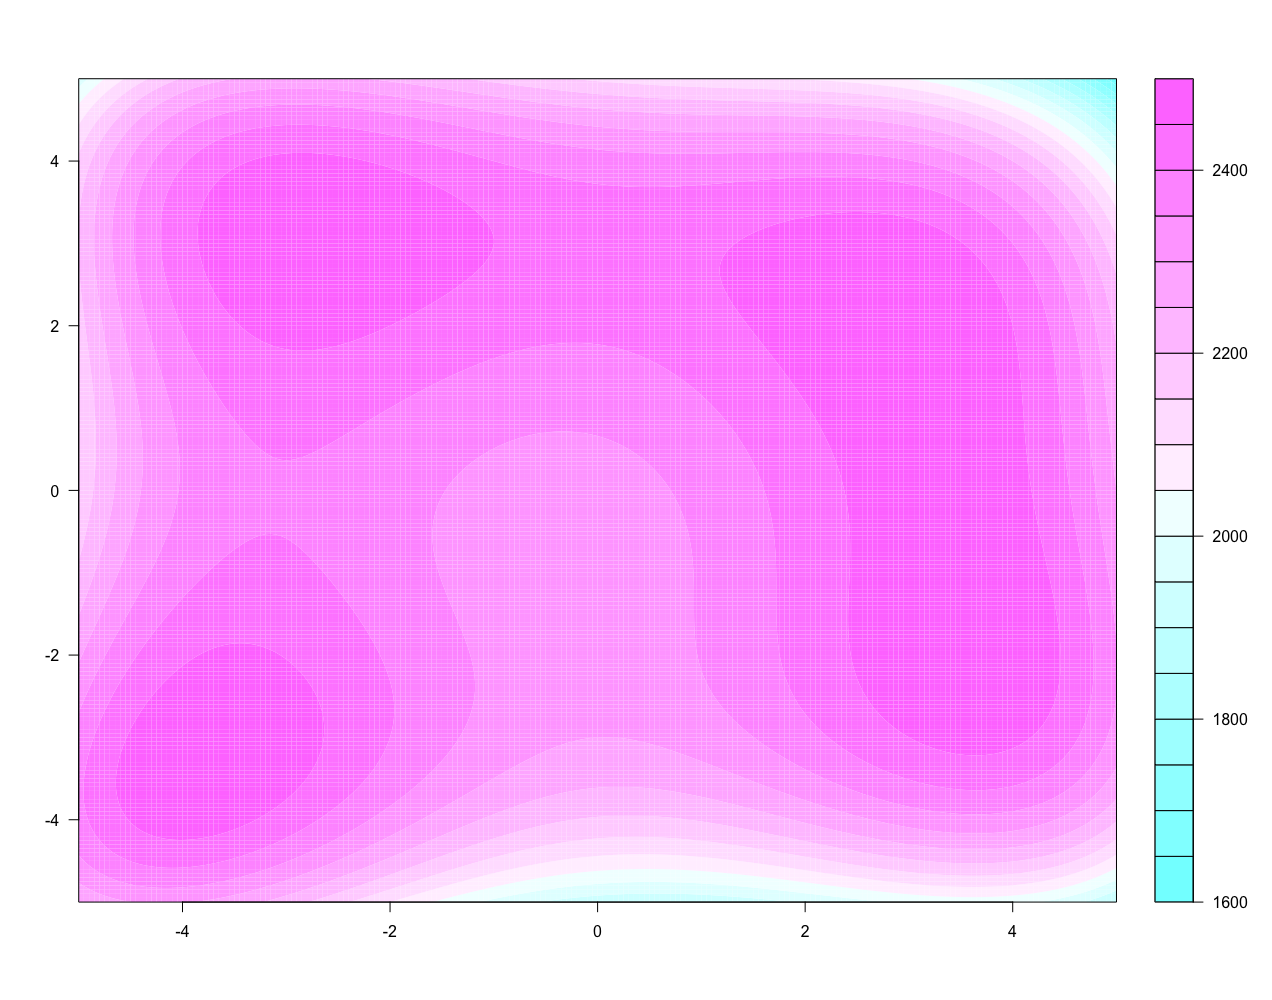
\includegraphics[width= 12cm, height = 10cm]{himmelblau.png}
	\caption{Contour plot of customized Himmelblau' s function.}
	\label{fig:ContourPlotCustomizedHimmelblauFunction}
\end{figure}
 
\subparagraph{Parabolic Function} Parabolic function is a multi-modal function. The function is defined by: 

\begin{equation}
f(x, y) = (x^2 + y^2)
\end{equation}

It's domain is $x = (-10, 10)$ and $y = (-10, 10)$.

In this thesis our aim is to maximize. In order to do this we have inverted the function as follow :

\begin{equation}
f(x, y) = -(x^2 + y^2)
\end{equation}

and we have picked it up of $3560$ units in order to have as less as possible negative values. So the final adopted function is :

\begin{equation}
f(x, y) = -(x^2 + y^2) + 3560
\end{equation}

This function has its local maximum in $f(x, y) = 3560$ and its minimum in $f(x, y) = 2560$.

In order to represent this function using {\tt JPanel} we mapped it in a space of $600 \times 600$ pixels and we properly rotated it. The resulting contour plot is the one represented in figure ~\ref{fig:ContourPlotCustomizedParabolicFunction} 

\begin{figure}[h!]
	\centering
	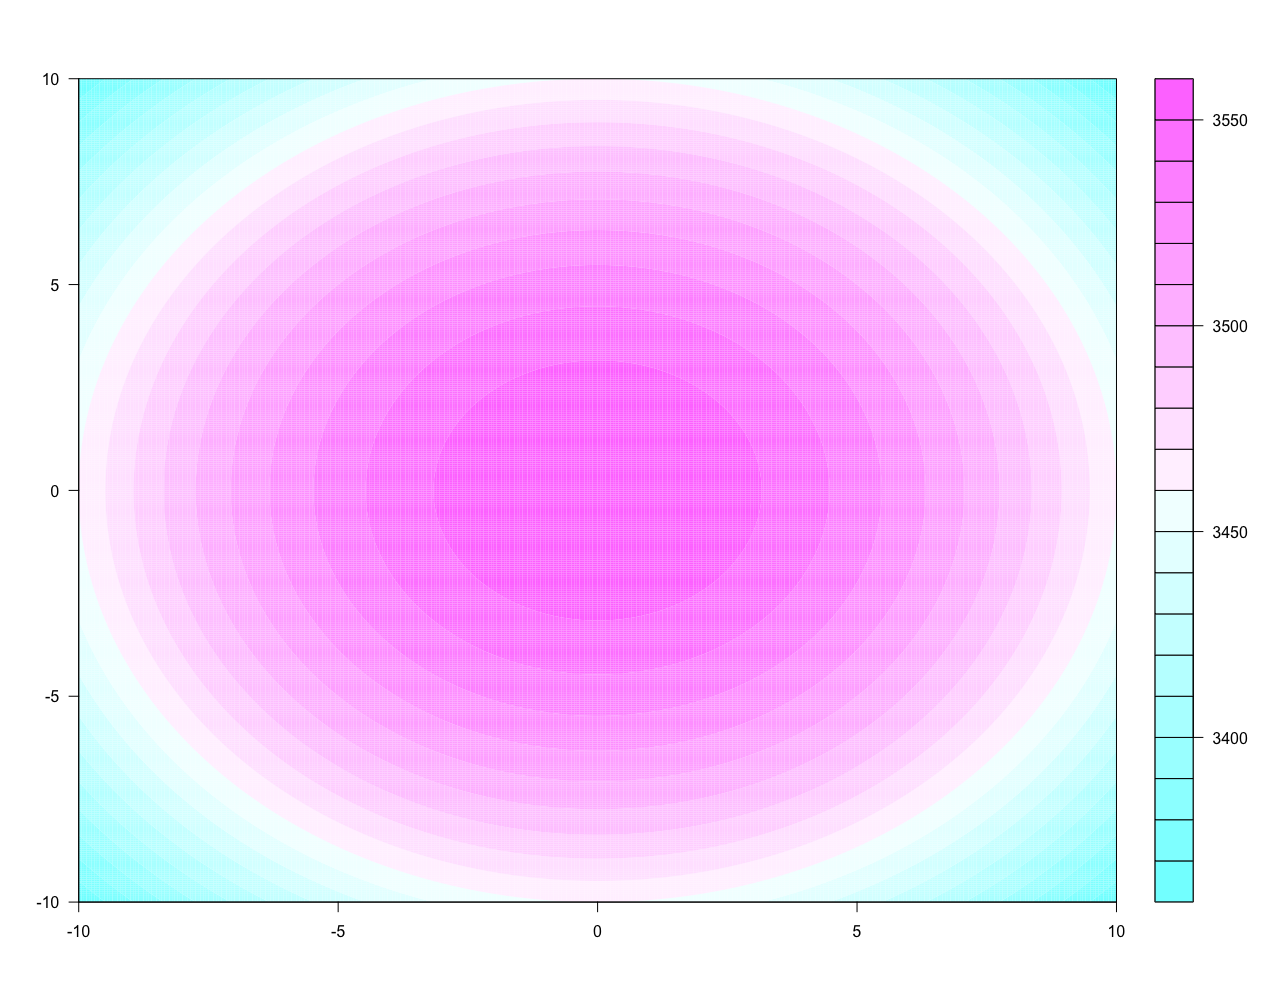
\includegraphics[width= 10cm, height = 10cm]{parabolic.png}
	\caption{Contour plot of customized Parabolic Function.}
	\label{fig:ContourPlotCustomizedParabolicFunction}
\end{figure}

\subparagraph{Beale Function} In mathematical optimization, Beale Function is a continuous, multi-modal function defined on a two-dimensional space. The function is defined by: 

\begin{equation}
f(x, y) = (1.5 - x + xy)^2 + (2.25 - x + xy^2)^2 + (2.625 - x + xy^3)^2
\end{equation}

The function can be defined on any input domain but it is usually evaluated on $x \in [-4.5, 4.5]$ and $y \in [-4.5, 4.5]$. \\

It has one global minimum at: $f(x, y) = 0$.

\begin{figure}[h!]
	\centering
	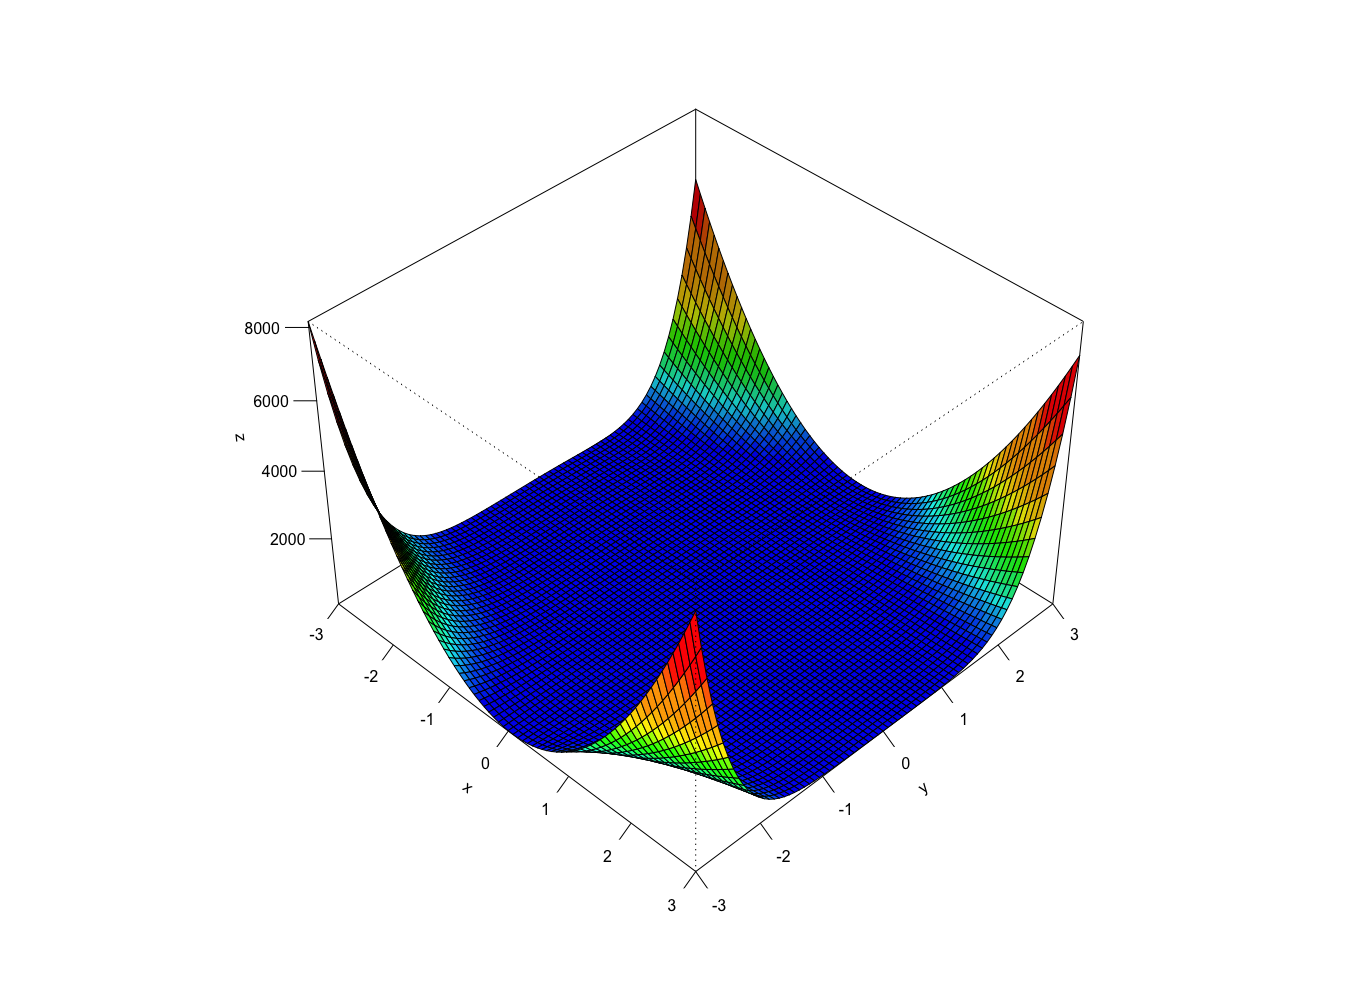
\includegraphics[width= 15cm, height = 12cm]{originalBeale.png}
	\caption{Original Beale Function.}
	\label{fig:OriginalBealeFunction}
\end{figure}

In this thesis our aim is to maximize. In order to do this we have inverted the function as

\begin{equation}
f(x, y) = -((1.5 - x + xy)^2 + (2.25 - x + xy^2)^2 + (2.625 - x + xy^3)^2)
\end{equation}

and we have picked it up of $2000$ units in order to have as less as possible negative values. So the final adopted function is :

\begin{equation}
f(x, y) = -((1.5 - x + xy)^2 + (2.25 - x + xy^2)^2 + (2.625 - x + xy^3)^2) + 2000
\end{equation}

We have also restricted the domain as $x = (-3, 3)$ and $y = (-3, 3)$. \\

This customized function has its local maximum in $f(x, y) = 1000$ and its minimum in $f(x, y) = 2000$.

\begin{figure}[h!]
	\centering
	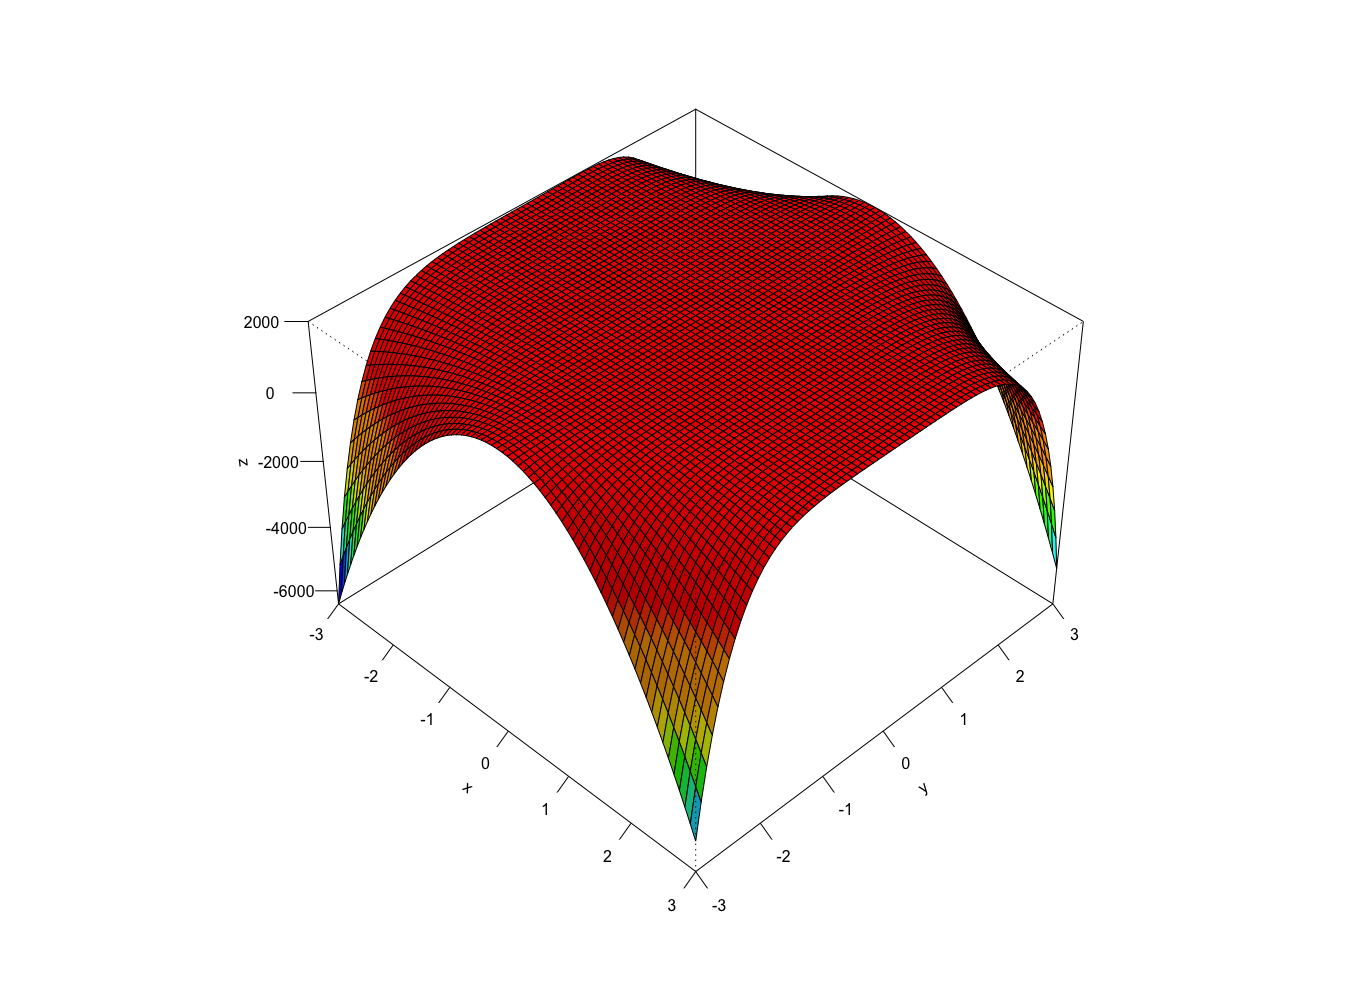
\includegraphics[width= 12cm, height = 10cm]{customizedBeale.png}
	\caption{Customized Beale Function.}
	\label{fig:CustomizedBealeFunction}
\end{figure}

In order to represent this function using {\tt JPanel} we mapped it in a space of $600 \times 600$ pixels and we properly rotated it. The resulting contour plot is the one represented in figure ~\ref{fig:ContourPlotCustomizedBealeFunction} 

\begin{figure}[h!]
	\centering
	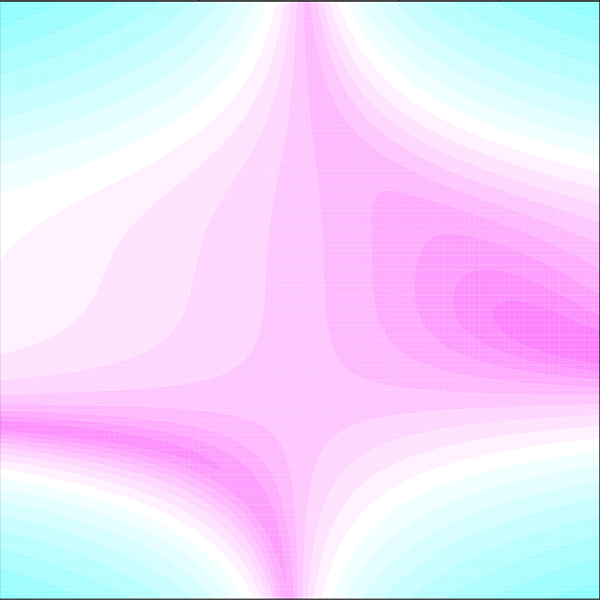
\includegraphics[width= 10cm, height = 10cm]{beale.png}
	\caption{Contour plot of customized Beale Function.}
	\label{fig:ContourPlotCustomizedBealeFunction}
\end{figure}

\subparagraph{Styblinski-Tang Function} In mathematical optimization, Styblinski Function is a continuous, multi-modal function defined on a two-dimensional space. The function is defined by :

\begin{equation}
	f(x, y) = (x^4 - 16 * x^2 + 5 * x) + (y^4 - 16 * y^2 + 5 * y)
\end{equation}

The function can be defined on any input domain but it is usually evaluated on $x \in [-5, 5]$ and $y \in [-5, 5]$.

\begin{figure}[h!]
	\centering
	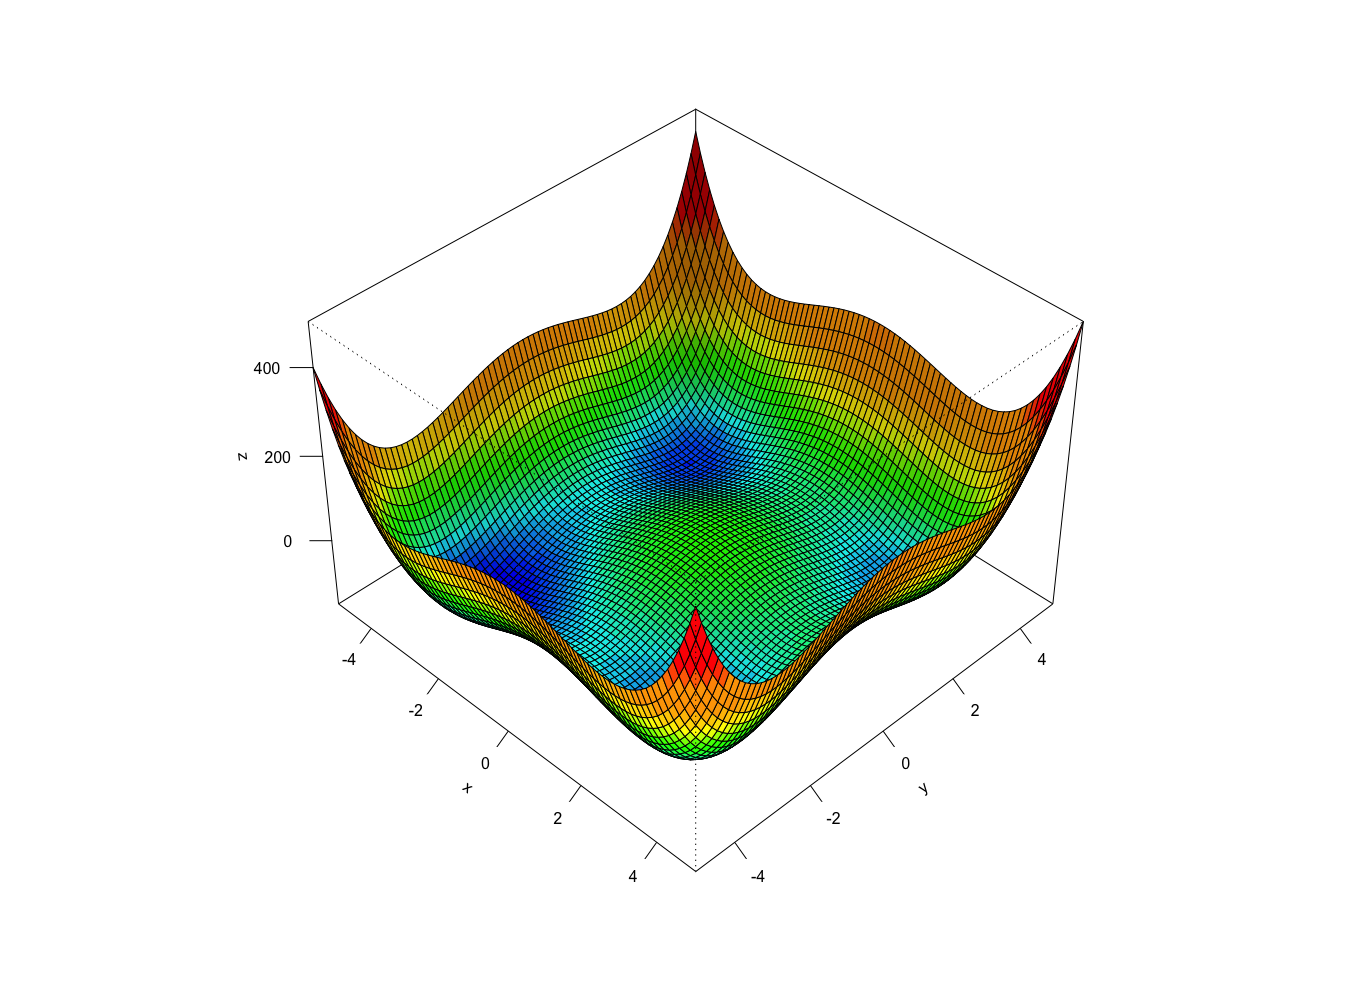
\includegraphics[width= 14.5cm, height = 13cm]{classicalStyblinski.png}
	\caption{Classical Styblinski-Tang Function.}
	\label{fig:ClassicalStyblinskiFunction}
\end{figure}

In this thesis our aim is to maximize. In order to do this we have inverted the function as

\begin{equation}
f(x, y) = -((x^4 - 16 * x^2 + 5 * x) + (y^4 - 16 * y^2 + 5 * y))
\end{equation}

and we have picked it up of $5000$ units in order to has as less as possible negative values. So the final adopted function is: 

\begin{equation}
f(x, y) = -((x^4 - 16 * x^2 + 5 * x) + (y^4 - 16 * y^2 + 5 * y)) + 5000
\end{equation}

This customized function has its local maximum in $f(x, y) = 5156.6638$ and its local minimum in $f(x, y) = 4500$. 

\begin{figure}[h!]
	\centering
	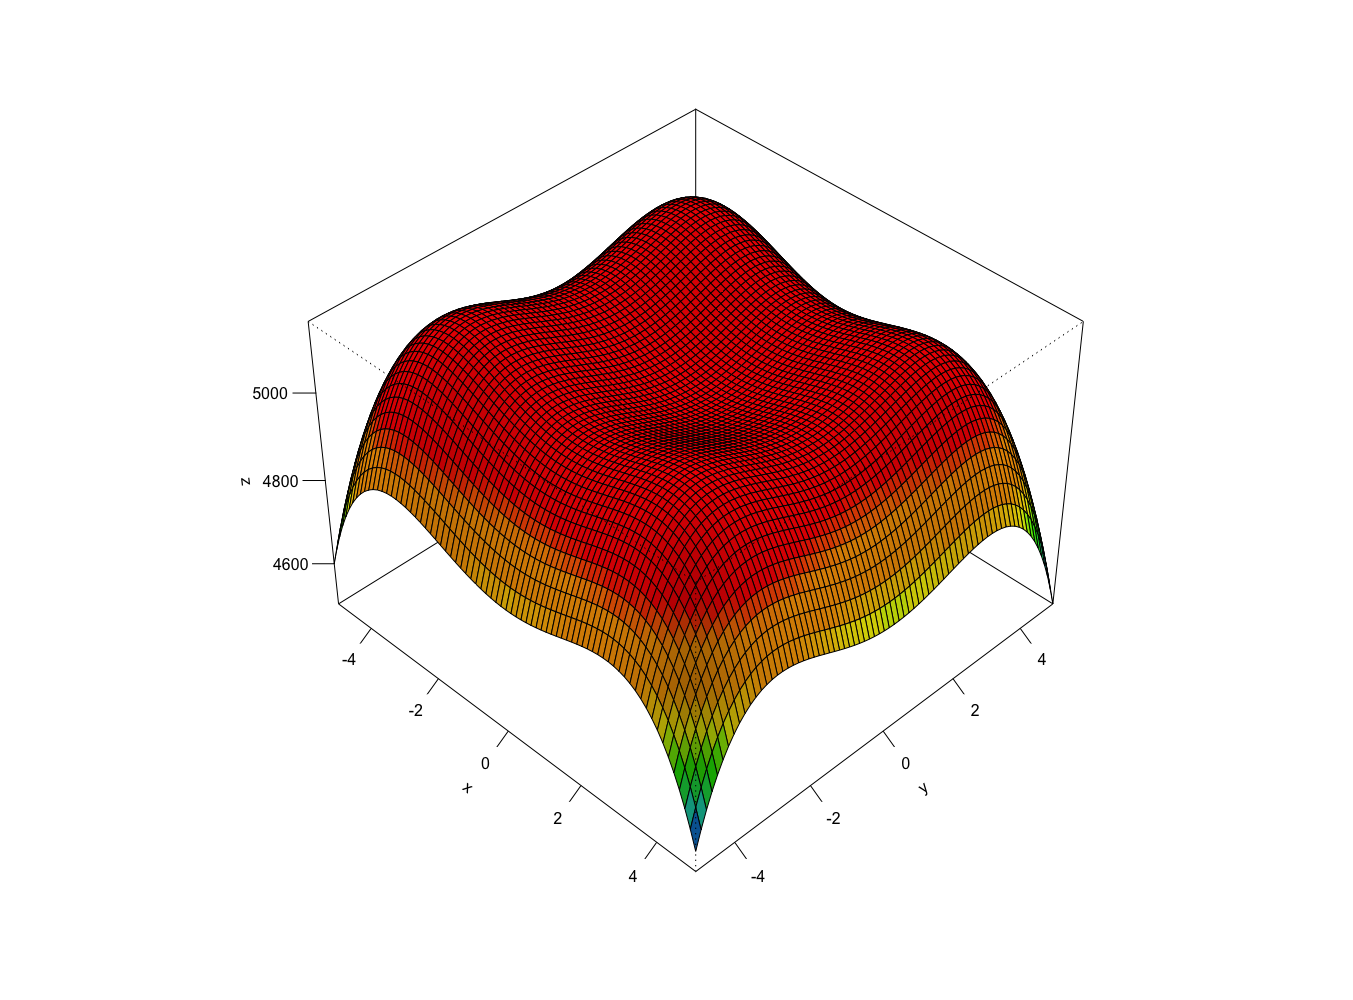
\includegraphics[width= 9cm, height = 9cm]{customizedStyblinski.png}
	\caption{Customized Styblinski-Tang Function.}
	\label{fig:CustumizedStyblinskiFunction}
\end{figure}

In order to represent this function using {\tt JPanel} we mapped its in a space of $600 \times 600$ pixels and we properly rotated its. The resulting contour plot is the one represented in figure ~\ref{fig:ContourStyblinskiFunction}.

\begin{figure}[h!]
	\centering
	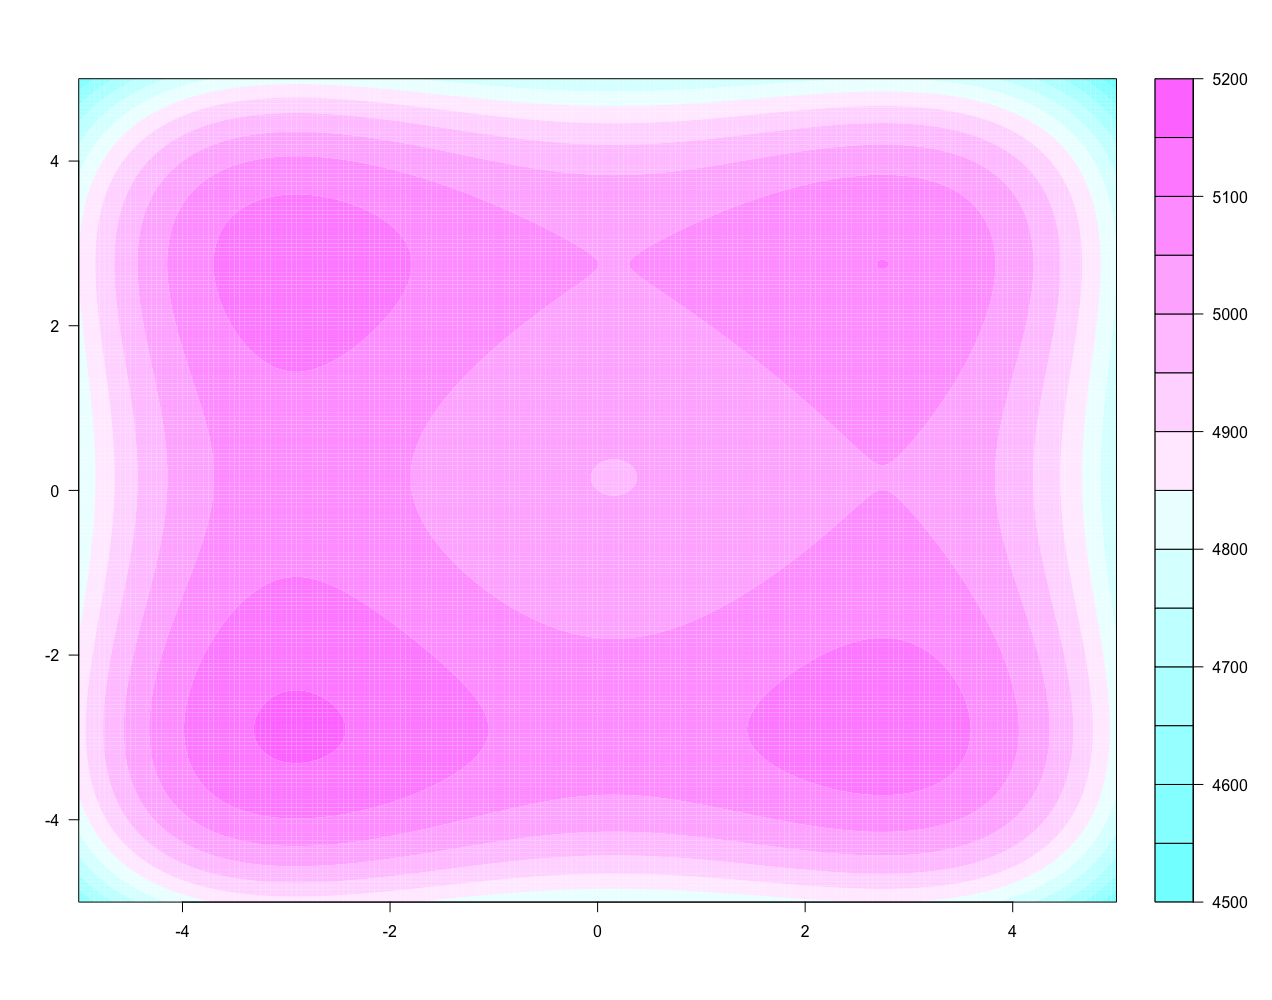
\includegraphics[width= 5cm, height = 5cm]{styblinski.png}
	\caption{Contour plot of customized Styblinski Function.}
	\label{fig:ContourStyblinskiFunction}
\end{figure}






